\documentclass[12pt,a4paper]{article}

% ─────────────────────────────────────────────
%  PACKAGES
% ─────────────────────────────────────────────
\usepackage{amsmath,amssymb}
\usepackage[margin=2.5cm]{geometry}
\usepackage{booktabs}
\usepackage{xcolor}
\usepackage{hyperref}
\usepackage{listings}
\usepackage{pgfplots}
\pgfplotsset{compat=1.18}
\usepackage[most,breakable]{tcolorbox}
\tcbuselibrary{skins,breakable}
\usepackage{enumitem}
\usepackage{fancyhdr}
\usepackage{tikz}
\usepackage{array}

% ─────────────────────────────────────────────
%  TCOLORBOX ENVIRONMENTS
% ─────────────────────────────────────────────
\newtcolorbox{curiositybox}[1]{colback=yellow!10, colframe=orange!80!black,
  fonttitle=\bfseries, title=#1, breakable}
\newtcolorbox{infobox}[1]{colback=blue!5, colframe=blue!60!black,
  fonttitle=\bfseries, title=#1, breakable}
\newtcolorbox{mistakebox}[1]{colback=red!5, colframe=red!60!black,
  fonttitle=\bfseries, title=#1, breakable}
\newtcolorbox{learnbox}[1]{colback=green!5, colframe=green!60!black,
  fonttitle=\bfseries, title=#1, breakable}

% ─────────────────────────────────────────────
%  LISTINGS SETUP (Python)
% ─────────────────────────────────────────────
\lstset{language=Python, basicstyle=\ttfamily\small,
        keywordstyle=\color{blue}, commentstyle=\color{gray},
        stringstyle=\color{red}, showstringspaces=false,
        breaklines=true, frame=single}

% ─────────────────────────────────────────────
%  FANCYHDR
% ─────────────────────────────────────────────
\pagestyle{fancy}
\fancyhf{}
\lhead{Topic 10: Contour Integration}
\rhead{Unit II --- Complex Variables}
\cfoot{\thepage}

% ─────────────────────────────────────────────
%  TITLE
% ─────────────────────────────────────────────
\title{\textbf{Topic 10: Contour Integration}\\[6pt]
       \large Unit II --- Complex Variable: Integration\\[4pt]
       \normalsize Complex Variables and Special Functions\\
       JNTUA College of Engineering (Autonomous)}
\author{}
\date{}

% ─────────────────────────────────────────────
\begin{document}
\maketitle
\tableofcontents
\newpage

% ═══════════════════════════════════════════════
%  OPENING HOOK
% ═══════════════════════════════════════════════
\begin{curiositybox}{Hook}
If a line integral follows any curve, then a contour integral is the next big step:
the curve may close into a loop. Once the path closes, extraordinary theorems begin
to appear --- and they become the foundation of complex integration.
\end{curiositybox}

% ═══════════════════════════════════════════════
\section{From Line Integral to Contour Integral}
% ═══════════════════════════════════════════════

In the previous topic we evaluated \(\int_C f(z)\,dz\) along a smooth arc $C$
from a start point to an end point. The key generalisation is to allow the path
to \emph{close}: the end point coincides with the start point, forming a
\emph{loop}. Such closed paths are called \textbf{contours}, and the integral
around them is written with the closed-path symbol $\oint$.

\begin{center}
\begin{tabular}{@{}lll@{}}
\toprule
Concept & Line Integral & Contour Integral \\
\midrule
Path & Open arc from $z_0$ to $z_1$ & Closed loop $C$ (start $=$ end) \\
Notation & $\displaystyle\int_C f(z)\,dz$ & $\displaystyle\oint_C f(z)\,dz$ \\
Path class & Piecewise smooth curve & Piecewise smooth, closed, rectifiable \\
Special power & Measures path dependence & Unlocks Cauchy's theorem \& residues \\
\bottomrule
\end{tabular}
\end{center}

\begin{learnbox}{Key Idea}
Closing a path transforms a line integral into a contour integral. This small
change has enormous consequences: it enables Cauchy's theorem, the residue
theorem, and the evaluation of real definite integrals via complex methods.
\end{learnbox}

% ═══════════════════════════════════════════════
\section{Definition of Contour and Contour Integral}
% ═══════════════════════════════════════════════

\begin{infobox}{Definitions}
\textbf{Contour.} A \emph{contour} $C$ in the complex plane is a piecewise smooth
arc, i.e.\ a finite union of smooth arcs joined end-to-end.

\medskip
\textbf{Simple contour.} A contour that does not cross itself (no
self-intersections), except possibly at the endpoints.

\medskip
\textbf{Closed contour.} A contour whose terminal point coincides with its
initial point.

\medskip
\textbf{Simple closed contour (Jordan curve).} A closed contour with no
self-intersections other than the shared start/end point.

\medskip
\textbf{Positively oriented contour.} A simple closed contour traversed
\emph{counterclockwise} (CCW). The interior of the curve lies to the
\emph{left} as one travels along $C$. Clockwise traversal is called
\emph{negatively oriented}.

\medskip
\textbf{Contour integral.} Let $f$ be a continuous function on a contour $C$
parametrised by $z(t)$, $a \le t \le b$. The \emph{contour integral} of $f$
along $C$ is
\[
  \oint_C f(z)\,dz = \int_a^b f\!\bigl(z(t)\bigr)\,z'(t)\,dt.
\]
The value is the same for any smooth reparametrisation that preserves
orientation.
\end{infobox}

\begin{learnbox}{Remember}
``Positively oriented'' always means counterclockwise for simple closed contours.
Reversing orientation multiplies the integral by $-1$.
\end{learnbox}

% ═══════════════════════════════════════════════
\section{Standard Contours}
% ═══════════════════════════════════════════════

\begin{infobox}{Common Contours in Complex Analysis}
\begin{enumerate}[leftmargin=1.5em]
\item \textbf{Circle} $|z - z_0| = r$: $z(t) = z_0 + re^{it}$, $t \in [0,2\pi]$ (CCW).
\item \textbf{Upper semicircle} of radius $R$: $z(t) = Re^{it}$, $t \in [0,\pi]$.
\item \textbf{Lower semicircle} of radius $R$: $z(t) = Re^{it}$, $t \in [\pi,2\pi]$.
\item \textbf{Rectangle} with vertices $a, b, b+id, a+id$: four straight-line
      segments traversed CCW.
\item \textbf{Triangle}: three straight-line segments; parametrize each side
      separately.
\item \textbf{Piecewise contour}: a finite union of arcs and segments joined end-to-end.
\end{enumerate}
\end{infobox}

\subsection*{Diagram: Standard Contour Types}

\begin{center}
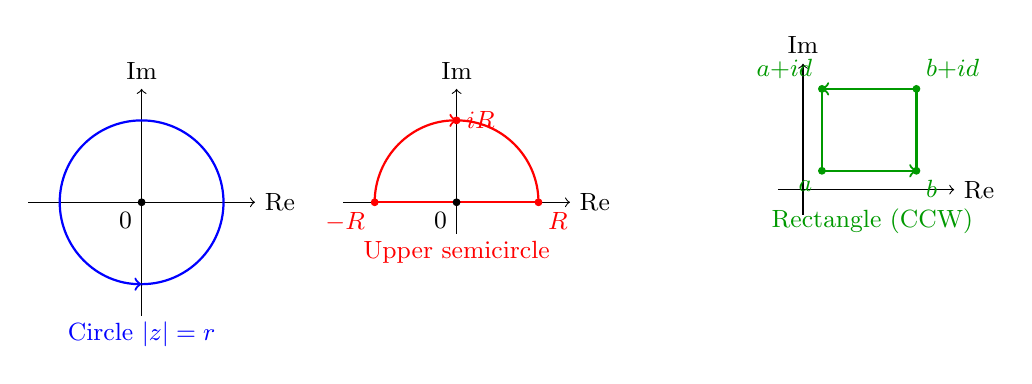
\begin{tikzpicture}[scale=0.80]
  % ---- Full circle ----
  \draw[->] (-1.8,0)--(1.8,0) node[right]{\small Re};
  \draw[->] (0,-1.8)--(0,1.8) node[above]{\small Im};
  \draw[->,blue,thick] (1.3,0) arc (0:270:1.3);
  \draw[blue,thick] (1.3,0) arc (0:-90:1.3);
  \node[blue] at (0,-2.1) {\small Circle $|z|=r$};
  \filldraw[black] (0,0) circle (1.5pt) node[below left]{\small $0$};

  % ---- Upper semicircle (shifted right) ----
  \begin{scope}[xshift=5cm]
    \draw[->] (-1.8,0)--(1.8,0) node[right]{\small Re};
    \draw[->] (0,-0.5)--(0,1.8) node[above]{\small Im};
    \draw[->,red,thick] (-1.3,0) arc (180:90:1.3);
    \draw[red,thick] (0,1.3) arc (90:0:1.3);
    \draw[red,thick] (1.3,0) -- (-1.3,0);
    \node[red] at (0,-0.8) {\small Upper semicircle};
    \filldraw[black] (0,0) circle (1.5pt) node[below left]{\small $0$};
    \filldraw[red] (1.3,0) circle (1.5pt) node[below right]{\small $R$};
    \filldraw[red] (-1.3,0) circle (1.5pt) node[below left]{\small $-R$};
    \filldraw[red] (0,1.3) circle (1.5pt) node[right]{\small $iR$};
  \end{scope}

  % ---- Rectangle (shifted right more) ----
  \begin{scope}[xshift=10.5cm, yshift=0.2cm]
    \draw[->] (-0.4,0)--(2.4,0) node[right]{\small Re};
    \draw[->] (0,-0.4)--(0,2.0) node[above]{\small Im};
    \draw[->,green!60!black,thick] (0.3,0.3)--(1.8,0.3);
    \draw[green!60!black,thick] (1.8,0.3)--(1.8,1.6);
    \draw[->,green!60!black,thick] (1.8,1.6)--(0.3,1.6);
    \draw[green!60!black,thick] (0.3,1.6)--(0.3,0.3);
    \node[green!60!black] at (1.1,-0.5) {\small Rectangle (CCW)};
    \filldraw[green!60!black] (0.3,0.3) circle (1.5pt) node[below left]{\small $a$};
    \filldraw[green!60!black] (1.8,0.3) circle (1.5pt) node[below right]{\small $b$};
    \filldraw[green!60!black] (1.8,1.6) circle (1.5pt) node[above right]{\small $b{+}id$};
    \filldraw[green!60!black] (0.3,1.6) circle (1.5pt) node[above left]{\small $a{+}id$};
  \end{scope}
\end{tikzpicture}
\end{center}

\begin{learnbox}{Takeaway}
Most contour integration problems in B.Tech use circles and upper semicircles.
Knowing their standard parametrizations by memory saves significant calculation time.
\end{learnbox}

% ═══════════════════════════════════════════════
\section{Orientation and Its Effect}
% ═══════════════════════════════════════════════

\begin{infobox}{Orientation Rule}
Let $-C$ denote the contour $C$ traversed in the \emph{opposite} direction.
Then:
\[
  \oint_{-C} f(z)\,dz = -\oint_C f(z)\,dz.
\]
Geometrically: counterclockwise (positive) vs.\ clockwise (negative).
The modulus $\left|\oint_C f(z)\,dz\right|$ is unchanged; only the sign flips.
\end{infobox}

\textbf{Why it matters.} Many textbook problems specify ``integrate $C$
clockwise.'' You can convert to the standard CCW form, evaluate the integral,
then negate the result. This avoids reworking the parametrization from scratch.

\begin{center}
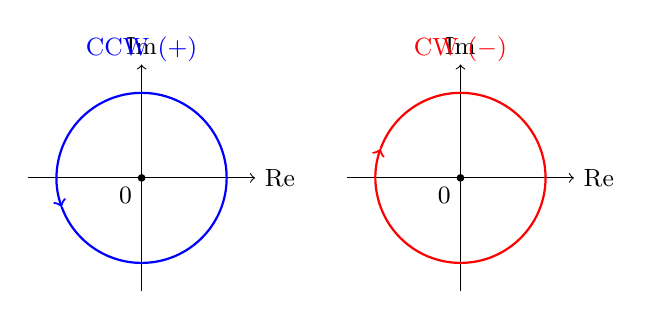
\begin{tikzpicture}[scale=0.9]
  % CCW circle
  \draw[->] (-1.6,0)--(1.6,0) node[right]{\small Re};
  \draw[->] (0,-1.6)--(0,1.6) node[above]{\small Im};
  \draw[->,blue,thick] (1.2,0) arc (0:200:1.2);
  \draw[blue,thick] (1.2,0) arc (0:-160:1.2);
  \node[blue,above] at (0,1.5) {\small CCW (+)};
  \filldraw[black] (0,0) circle (1.3pt) node[below left]{\small $0$};

  % CW circle (shifted right)
  \begin{scope}[xshift=4.5cm]
    \draw[->] (-1.6,0)--(1.6,0) node[right]{\small Re};
    \draw[->] (0,-1.6)--(0,1.6) node[above]{\small Im};
    \draw[->,red,thick] (1.2,0) arc (0:-200:1.2);
    \draw[red,thick] (1.2,0) arc (0:160:1.2);
    \node[red,above] at (0,1.5) {\small CW $(-)$};
    \filldraw[black] (0,0) circle (1.3pt) node[below left]{\small $0$};
  \end{scope}
\end{tikzpicture}
\end{center}

\begin{learnbox}{Key Result}
Reversing the direction of traversal negates the contour integral.
Always note the orientation before beginning any calculation.
\end{learnbox}

% ═══════════════════════════════════════════════
\section{Evaluating Contour Integrals by Parametrization}
% ═══════════════════════════════════════════════

\begin{infobox}{Method}
To evaluate $\int_C f(z)\,dz$:
\begin{enumerate}[leftmargin=1.8em]
  \item Write a parametrization $z = z(t)$, $t \in [a,b]$.
  \item Compute $dz = z'(t)\,dt$.
  \item Substitute $f(z(t))$ and $z'(t)$ into the integral and evaluate
        $\int_a^b f(z(t))\,z'(t)\,dt$ as a real integral.
\end{enumerate}
\end{infobox}

\subsection*{Model Parametrization 1: Unit Circle}

Let $C : |z| = 1$ traversed CCW.
\[
  z(t) = e^{it} = \cos t + i\sin t, \quad t \in [0,2\pi], \quad z'(t) = ie^{it}.
\]

\subsection*{Model Parametrization 2: Upper Semicircle of Radius $R$}

Let $C_R$ be the upper semicircle $|z|=R$, $\operatorname{Im}(z)\ge 0$,
traversed from $-R$ to $R$ via the top.
\[
  z(t) = Re^{it}, \quad t \in [0,\pi], \quad z'(t) = iRe^{it}.
\]

\subsection*{Model Parametrization 3: Straight-Line Segment from $z_0$ to $z_1$}

\[
  z(t) = (1-t)z_0 + t\,z_1, \quad t \in [0,1], \quad z'(t) = z_1 - z_0.
\]

\begin{learnbox}{Standard Parametrizations}
Memorise these three: unit circle, upper semicircle of radius $R$, and the linear
interpolation for a straight segment. They cover the vast majority of B.Tech problems.
\end{learnbox}

% ═══════════════════════════════════════════════
\section{Connection with Path Dependence}
% ═══════════════════════════════════════════════

\begin{infobox}{Path Dependence}
A complex integral $\int_C f(z)\,dz$ is \emph{path independent} in a domain
$D$ if and only if $f$ is analytic in $D$ and $D$ is simply connected --- a
fact established by Cauchy's theorem (Topic 11).

When $f$ has singularities inside a closed contour, the value of the integral
around that contour is generally \emph{non-zero} and depends on the singularity
structure, not just the shape of the contour.
\end{infobox}

\textbf{Example of path dependence.} Consider $f(z) = 1/z$. Integrating over
the unit circle (which encloses the singularity $z=0$) gives $2\pi i$, while
integrating over any closed path that does \emph{not} enclose $z=0$ gives $0$.
This contrast motivates Cauchy's theorem and the residue theorem.

\begin{learnbox}{Why This Matters}
Path dependence is directly linked to singularities enclosed by the contour.
If $f$ is analytic everywhere inside $C$, the integral is zero. If not, we need
the residue theorem --- which we will study in Topics 17--18.
\end{learnbox}

% ═══════════════════════════════════════════════
\section{Worked Examples}
% ═══════════════════════════════════════════════

% ────────────────────────────────────────────────
\subsection*{Example 1: \(\oint_C z\,dz\) over the Unit Circle}
% ────────────────────────────────────────────────

\textbf{Problem.} Evaluate $\displaystyle\oint_C z\,dz$ where $C : |z|=1$, CCW.

\textbf{Solution.} Parametrize: $z(t)=e^{it}$, $z'(t)=ie^{it}$, $t\in[0,2\pi]$.
\begin{align*}
\oint_C z\,dz &= \int_0^{2\pi} e^{it} \cdot ie^{it}\,dt
              = i\int_0^{2\pi} e^{2it}\,dt
              = i\left[\frac{e^{2it}}{2i}\right]_0^{2\pi}
              = \frac{1}{2}\left[e^{4\pi i}-e^{0}\right]
              = \frac{1}{2}(1-1) = 0.
\end{align*}

\begin{learnbox}{Result}
$\oint_C z\,dz = 0$ over any closed contour. This confirms that $f(z)=z$ is entire
(analytic everywhere), so by Cauchy's theorem the closed integral is zero.
\end{learnbox}

% ────────────────────────────────────────────────
\subsection*{Example 2: \(\oint_C \frac{1}{z}\,dz\) over the Unit Circle}
% ────────────────────────────────────────────────

\textbf{Problem.} Evaluate $\displaystyle\oint_C \frac{1}{z}\,dz$ where $C : |z|=1$, CCW.

\textbf{Solution.} $z(t)=e^{it}$, $z'(t)=ie^{it}$, $t\in[0,2\pi]$.
\begin{align*}
\oint_C \frac{1}{z}\,dz &= \int_0^{2\pi} \frac{1}{e^{it}} \cdot ie^{it}\,dt
                         = \int_0^{2\pi} i\,dt
                         = i\cdot 2\pi = 2\pi i.
\end{align*}

\begin{learnbox}{Result}
$\oint_C \frac{1}{z}\,dz = 2\pi i$. This is the cornerstone result of complex
analysis; the singularity at $z=0$ inside $C$ produces the non-zero value.
\end{learnbox}

% ────────────────────────────────────────────────
\subsection*{Example 3: \(\oint_C z^2\,dz\) over the Circle $|z|=3$}
% ────────────────────────────────────────────────

\textbf{Problem.} Evaluate $\displaystyle\oint_C z^2\,dz$ where $C : |z|=3$, CCW.

\textbf{Solution.} $z(t)=3e^{it}$, $z'(t)=3ie^{it}$, $t\in[0,2\pi]$.
\begin{align*}
\oint_C z^2\,dz &= \int_0^{2\pi} (3e^{it})^2 \cdot 3ie^{it}\,dt
                = \int_0^{2\pi} 9e^{2it}\cdot 3ie^{it}\,dt
                = 27i\int_0^{2\pi} e^{3it}\,dt \\
                &= 27i\left[\frac{e^{3it}}{3i}\right]_0^{2\pi}
                = 9\left[e^{6\pi i} - 1\right]
                = 9(1-1) = 0.
\end{align*}

\begin{learnbox}{Result}
$z^2$ is entire, so the closed integral is zero regardless of the radius of the circle.
\end{learnbox}

% ────────────────────────────────────────────────
\subsection*{Example 4: Piecewise Contour --- Triangle}
% ────────────────────────────────────────────────

\textbf{Problem.} Evaluate $\displaystyle\int_C \overline{z}\,dz$ where $C$ is
the triangle with vertices $0,\;1,\;1+i$, traversed in this order (CCW sense).

\textbf{Solution.} Split $C = C_1 \cup C_2 \cup C_3$.

\medskip
\textbf{Segment $C_1$: $0 \to 1$.}
$z(t)=t$, $t\in[0,1]$, $\overline{z}=t$, $dz=dt$.
\[\int_{C_1}\overline{z}\,dz = \int_0^1 t\,dt = \frac{1}{2}.\]

\textbf{Segment $C_2$: $1 \to 1+i$.}
$z(t)=1+it$, $t\in[0,1]$, $\overline{z}=1-it$, $dz=i\,dt$.
\[\int_{C_2}\overline{z}\,dz = \int_0^1 (1-it)\cdot i\,dt = \int_0^1(i+t)\,dt
= \left[it+\frac{t^2}{2}\right]_0^1 = i+\frac{1}{2}.\]

\textbf{Segment $C_3$: $1+i \to 0$.}
$z(t)=(1-t)(1+i)$, $t\in[0,1]$, $z'(t)=-(1+i)$,
$\overline{z}=(1-t)(1-i)$.
\[\int_{C_3}\overline{z}\,dz = \int_0^1 (1-t)(1-i)\cdot(-(1+i))\,dt
= -(1-i)(1+i)\int_0^1(1-t)\,dt = -2\cdot\frac{1}{2} = -1.\]

\textbf{Total:}
\[\int_C \overline{z}\,dz = \frac{1}{2} + \left(i+\frac{1}{2}\right) + (-1) = i.\]

\begin{learnbox}{Method}
For a piecewise contour, integrate over each smooth segment separately and add
the results. Keep track of the direction (increasing $t$) on every piece.
\end{learnbox}

% ────────────────────────────────────────────────
\subsection*{Example 5: Orientation Reversal}
% ────────────────────────────────────────────────

\textbf{Problem.} Given $\displaystyle\oint_C \frac{1}{z}\,dz = 2\pi i$ for $C: |z|=1$ CCW,
find the value for the same circle traversed \emph{clockwise}.

\textbf{Solution.} Let $-C$ denote the unit circle with clockwise orientation.
By the orientation reversal rule:
\[
  \oint_{-C}\frac{1}{z}\,dz = -\oint_C\frac{1}{z}\,dz = -2\pi i.
\]

\begin{learnbox}{Result}
Changing orientation from CCW to CW negates the value of the integral.
No re-parametrization is needed once the CCW value is known.
\end{learnbox}

% ────────────────────────────────────────────────
\subsection*{Example 6: Integral of $\frac{1}{z^2}$ over a Circle Not Centred at the Origin}
% ────────────────────────────────────────────────

\textbf{Problem.} Evaluate $\displaystyle\oint_C \frac{1}{(z-2)^2}\,dz$
where $C: |z-2|=1$, CCW.

\textbf{Solution.} The circle is centred at $z_0=2$ with radius $1$.
Parametrize: $z(t)=2+e^{it}$, $z'(t)=ie^{it}$, $t\in[0,2\pi]$.
Then $z-2=e^{it}$, so $(z-2)^2=e^{2it}$.
\begin{align*}
\oint_C \frac{1}{(z-2)^2}\,dz &= \int_0^{2\pi} \frac{1}{e^{2it}}\cdot ie^{it}\,dt
= i\int_0^{2\pi} e^{-it}\,dt
= i\left[\frac{e^{-it}}{-i}\right]_0^{2\pi}
= \left[-e^{-it}\right]_0^{2\pi}
= -(1-1) = 0.
\end{align*}

\begin{learnbox}{Result}
$\oint_C (z-z_0)^n\,dz = 0$ for any integer $n \neq -1$ over a circle centred
at $z_0$. The special case $n=-1$ gives $2\pi i$.
\end{learnbox}

% ═══════════════════════════════════════════════
\section{Contour Catalogue Table (MANDATORY UPGRADE)}
% ═══════════════════════════════════════════════

\begin{infobox}{Contour Catalogue}
\renewcommand{\arraystretch}{1.35}
\begin{tabular}{@{}p{3.2cm}p{4.8cm}p{2.8cm}p{2.5cm}@{}}
\toprule
\textbf{Contour Type} & \textbf{Parametrization} & \textbf{Interval} & \textbf{Orientation} \\
\midrule
Full circle $|z-z_0|=r$ & $z(t)=z_0+re^{it}$ & $t\in[0,2\pi]$ & CCW (+) \\
Full circle (CW) & $z(t)=z_0+re^{-it}$ & $t\in[0,2\pi]$ & CW ($-$) \\
Upper semicircle $|z|=R$, $\operatorname{Im}(z)\ge0$ & $z(t)=Re^{it}$ & $t\in[0,\pi]$ & $-R \to R$ via top \\
Lower semicircle $|z|=R$, $\operatorname{Im}(z)\le0$ & $z(t)=Re^{-it}$ & $t\in[0,\pi]$ & $R \to -R$ via bottom \\
Straight segment $z_0\to z_1$ & $z(t)=(1-t)z_0+tz_1$ & $t\in[0,1]$ & $z_0 \to z_1$ \\
Indented semicircle (small, radius $\varepsilon$) & $z(t)=z_0+\varepsilon e^{i(\pi-t)}$ & $t\in[0,\pi]$ & CW (standard indent) \\
Rectangle vertices $a,b,b+id,a+id$ & Four segments: $a\to b$, $b\to b+id$, $b+id\to a+id$, $a+id\to a$ & $t\in[0,1]$ per side & CCW (+) \\
Triangle vertices $z_1,z_2,z_3$ & Three segments: $z_1\to z_2$, $z_2\to z_3$, $z_3\to z_1$ & $t\in[0,1]$ per side & CCW (+) \\
\bottomrule
\end{tabular}
\end{infobox}

\begin{learnbox}{Using the Catalogue}
Always identify the contour type first, then copy the standard parametrization
from this table. This avoids sign errors and incorrect angle ranges.
\end{learnbox}

% ═══════════════════════════════════════════════
\section{Excel Example (MANDATORY)}
% ═══════════════════════════════════════════════

\textbf{Goal.} Numerically approximate $\displaystyle\oint_C \frac{1}{z}\,dz$
over $C: |z|=1$ (CCW) by sampling $N=8$ points and using the trapezoidal rule.

\medskip
\textbf{Spreadsheet Setup.} In a new worksheet, create these columns:

\begin{center}
\renewcommand{\arraystretch}{1.25}
\begin{tabular}{@{}ccccccc@{}}
\toprule
\textbf{Col A} & \textbf{Col B} & \textbf{Col C} & \textbf{Col D}
& \textbf{Col E} & \textbf{Col F} & \textbf{Col G} \\
$k$ & $t_k$ & $\cos(t_k)$ & $\sin(t_k)$ & $\operatorname{Re}(f(z)z'(t))$
& $\operatorname{Im}(f(z)z'(t))$ & $\Delta t$ \\
\midrule
0 & 0 & 1.0000 & 0.0000 & 0.0000 & 1.0000 & 0.7854 \\
1 & 0.7854 & 0.7071 & 0.7071 & 0.0000 & 1.0000 & 0.7854 \\
2 & 1.5708 & 0.0000 & 1.0000 & 0.0000 & 1.0000 & 0.7854 \\
3 & 2.3562 & $-0.7071$ & 0.7071 & 0.0000 & 1.0000 & 0.7854 \\
4 & 3.1416 & $-1.0000$ & 0.0000 & 0.0000 & 1.0000 & 0.7854 \\
5 & 3.9270 & $-0.7071$ & $-0.7071$ & 0.0000 & 1.0000 & 0.7854 \\
6 & 4.7124 & 0.0000 & $-1.0000$ & 0.0000 & 1.0000 & 0.7854 \\
7 & 5.4978 & 0.7071 & $-0.7071$ & 0.0000 & 1.0000 & 0.7854 \\
\bottomrule
\end{tabular}
\end{center}

\textbf{Key Excel Formulas.}
\begin{itemize}[leftmargin=1.5em]
  \item \texttt{B2} (first $t_k$): \texttt{= 0}; \texttt{B3}: \texttt{= B2 + 2*PI()/8}
  \item \texttt{C2}: \texttt{= COS(B2)} \quad (real part of $z$)
  \item \texttt{D2}: \texttt{= SIN(B2)} \quad (imaginary part of $z$)
  \item For $f(z)=1/z$ and $z=e^{it}$, $f(z)z'(t)=i$:
        \texttt{E2 = 0} (real part constant $= 0$); \texttt{F2 = 1} (imaginary part $= 1$)
  \item Approximate $\operatorname{Im}$ of integral: \texttt{= SUMPRODUCT(F2:F9, G2:G9)}
        $\approx 8 \times 1.0000 \times 0.7854 = 6.2832 \approx 2\pi$.
\end{itemize}

\textbf{Interpretation.} The real part sums to $\approx 0$ and the imaginary
part sums to $\approx 2\pi \approx 6.2832$, confirming
$\oint_C \frac{1}{z}\,dz \approx 2\pi i$.

\begin{learnbox}{Numerical Verification}
Excel provides a quick sanity check for contour integral values. Increasing $N$
(number of sample points) improves accuracy and the result converges to $2\pi i$.
\end{learnbox}

% ═══════════════════════════════════════════════
\section{Python Example (MANDATORY)}
% ═══════════════════════════════════════════════

\textbf{Goal.} Plot the unit circle contour and numerically verify
$\oint_C \frac{1}{z}\,dz = 2\pi i$ using the trapezoidal rule with $N=1000$ points.

\begin{lstlisting}[language=Python]
import numpy as np
import matplotlib.pyplot as plt

# ── Contour: unit circle |z| = 1, CCW ──────────────────────────
N = 1000
t = np.linspace(0, 2 * np.pi, N, endpoint=False)
z = np.exp(1j * t)          # z(t) = e^(it)
dz = 1j * np.exp(1j * t) * (2 * np.pi / N)  # dz = i*e^(it)*dt

# ── Integrand f(z) = 1/z ───────────────────────────────────────
f = 1.0 / z

# ── Numerical integral (trapezoidal sum) ───────────────────────
integral = np.sum(f * dz)
print(f"Integral of 1/z over |z|=1: {integral:.6f}")
# Expected output: 0.000000 + 6.283185j  (i.e., 2*pi*i)

# ── Plot the contour ───────────────────────────────────────────
fig, ax = plt.subplots(figsize=(5, 5))
ax.plot(z.real, z.imag, 'b-', linewidth=2, label=r'$|z|=1$ (CCW)')
ax.plot(1, 0, 'go', markersize=8, label='Start/End $z=1$')
ax.axhline(0, color='k', linewidth=0.5)
ax.axvline(0, color='k', linewidth=0.5)
ax.set_xlabel('Re(z)')
ax.set_ylabel('Im(z)')
ax.set_title(r'Contour $|z|=1$, CCW')
ax.legend()
ax.set_aspect('equal')
ax.annotate('', xy=(0.05, 1.02), xytext=(-0.05, 1.02),
            arrowprops=dict(arrowstyle='->', color='blue', lw=1.5))
plt.tight_layout()
plt.savefig('contour_unit_circle.png', dpi=150)
plt.show()

# ── Verify for circle |z| = 3 (no singularity at 0 is inside) ─
z3 = 3 * np.exp(1j * t)
dz3 = 3j * np.exp(1j * t) * (2 * np.pi / N)
f_z2 = z3 ** 2
integral_z2 = np.sum(f_z2 * dz3)
print(f"Integral of z^2 over |z|=3: {integral_z2:.6f}")
# Expected output: approximately 0.000000+0.000000j  (Cauchy's theorem)
\end{lstlisting}

\textbf{Expected output:}
\begin{verbatim}
Integral of 1/z over |z|=1: 0.000000+6.283185j
Integral of z^2 over |z|=3: 0.000000+0.000000j
\end{verbatim}

\begin{learnbox}{Python Insight}
The numerical result confirms the theoretical value $2\pi i \approx 6.2832i$.
The second calculation confirms that $\oint_C z^2\,dz = 0$ when no singularity
exists inside $C$.
\end{learnbox}

% ═══════════════════════════════════════════════
\section{Viva Questions}
% ═══════════════════════════════════════════════

\begin{enumerate}[leftmargin=2em]

\item \textbf{Define a contour in the complex plane.}\\
A contour is a piecewise smooth arc in $\mathbb{C}$: a finite union of smooth
arcs joined end-to-end, each having a continuous nonzero derivative.

\item \textbf{What is a simple closed contour?}\\
A closed contour (start point $=$ end point) that does not cross itself at any
intermediate point. It divides the plane into a bounded interior and an
unbounded exterior (Jordan curve theorem).

\item \textbf{What is positive orientation of a contour?}\\
Counterclockwise (CCW) traversal such that the interior of the contour lies to
the left of the direction of travel.

\item \textbf{State the effect of reversing the orientation of a contour.}\\
$\oint_{-C} f(z)\,dz = -\oint_C f(z)\,dz$. The magnitude is unchanged; the sign
is negated.

\item \textbf{Write the standard parametrization of the circle $|z - z_0| = r$ (CCW).}\\
$z(t) = z_0 + re^{it}$, $t \in [0, 2\pi]$, so $dz = ire^{it}\,dt$.

\item \textbf{Evaluate $\oint_{|z|=1} z^n\,dz$ for integer $n$.}\\
$\oint_{|z|=1} z^n\,dz = 2\pi i$ if $n = -1$, and $= 0$ for all other integers
$n$. This follows from direct parametrization.

\item \textbf{What distinguishes a contour integral from a line integral in complex analysis?}\\
A contour integral is a line integral in the complex plane evaluated along a
directed piecewise smooth curve. The distinction is mainly notational: $\oint$
emphasizes a closed path, while $\int_C$ is used for open paths.

\item \textbf{Why does the contour integral of $1/z$ around a circle not enclosing the origin equal zero?}\\
If the singularity $z=0$ lies outside the contour, then $1/z$ is analytic
throughout the closed interior. By Cauchy's theorem (Topic 11), the integral is
zero.

\end{enumerate}

% ═══════════════════════════════════════════════
\section{Descriptive Questions}
% ═══════════════════════════════════════════════

\begin{enumerate}[leftmargin=2em]

\item \textbf{Define a contour integral and explain how it is evaluated by parametrization.
Give a fully worked example using $f(z) = z^2$ over the circle $|z|=2$.}

A contour integral $\int_C f(z)\,dz$ is evaluated by substituting a smooth
parametrization $z = z(t)$, computing $dz = z'(t)\,dt$, and evaluating the
resulting real integral. For $f(z) = z^2$, $C: |z|=2$: let $z(t) = 2e^{it}$,
$dz = 2ie^{it}\,dt$, $t \in [0,2\pi]$:
\[
\oint_C z^2\,dz = \int_0^{2\pi}4e^{2it}\cdot 2ie^{it}\,dt
= 8i\int_0^{2\pi}e^{3it}\,dt = 8i\cdot 0 = 0,
\]
since $\int_0^{2\pi}e^{3it}\,dt = 0$. The result is zero because $z^2$ is entire.

\item \textbf{Explain the concept of orientation of a contour. How does reversing
orientation affect the value of the integral? Illustrate with $\oint_C \frac{1}{z}\,dz$.}

Orientation refers to the direction of traversal. Positive (CCW) places the
interior to the left; negative (CW) places it to the right. For $C: |z|=1$ CCW,
$\oint_C \frac{1}{z}\,dz = 2\pi i$. For CW traversal,
$\oint_{-C}\frac{1}{z}\,dz = -2\pi i$. This is because the substitution
$t \to -t$ introduces a factor of $-1$ in $dz$.

\item \textbf{List and describe four standard contours used in complex integration.
For each, write its parametrization and the parameter interval.}

(i) Circle $|z|=r$: $z(t)=re^{it}$, $t\in[0,2\pi]$, CCW.
(ii) Upper semicircle: $z(t)=Re^{it}$, $t\in[0,\pi]$.
(iii) Straight segment from $a$ to $b$: $z(t)=a+t(b-a)$, $t\in[0,1]$.
(iv) Rectangle with vertices $0,\,L,\,L+id,\,id$ (CCW): four straight segments
each parametrized linearly.

\item \textbf{Evaluate $\int_C \operatorname{Re}(z)\,dz$ along
(a) the straight line from $0$ to $1+i$, and (b) the arc of the unit circle
from $1$ to $i$. Comment on path dependence.}

(a) $z(t)=t(1+i)$, $\operatorname{Re}(z)=t$, $dz=(1+i)\,dt$:
$\int_0^1 t(1+i)\,dt = \frac{1+i}{2}$.

(b) $z(t)=e^{it}$, $t\in[0,\pi/2]$, $\operatorname{Re}(z)=\cos t$, $dz=ie^{it}\,dt$:
$\int_0^{\pi/2}\cos t\cdot ie^{it}\,dt = \int_0^{\pi/2}\cos t(i\cos t - \sin t)\,dt$.
Computing: real part $-\int_0^{\pi/2}\cos t\sin t\,dt = -\frac{1}{4}$;
imaginary part $i\int_0^{\pi/2}\cos^2 t\,dt = \frac{\pi i}{4}$.
Result: $-\frac{1}{4}+\frac{\pi i}{4}$.

The two results differ, confirming path dependence for $\operatorname{Re}(z)$,
which is not analytic.

\item \textbf{State and explain the formula for evaluating a piecewise contour integral.
Apply it to evaluate $\int_C (z+1)\,dz$ where $C$ consists of the segment from
$0$ to $2$ followed by the segment from $2$ to $2+2i$.}

For a piecewise contour $C = C_1 \cup C_2 \cup \cdots \cup C_n$:
$\int_C f\,dz = \int_{C_1} f\,dz + \int_{C_2} f\,dz + \cdots$

Segment $C_1$: $z=t$, $t\in[0,2]$, $dz=dt$:
$\int_0^2(t+1)\,dt = \left[\frac{t^2}{2}+t\right]_0^2 = 4$.

Segment $C_2$: $z=2+it$, $t\in[0,2]$, $dz=i\,dt$:
$\int_0^2(3+it)\cdot i\,dt = \int_0^2(3i-t)\,dt
= \left[3it-\frac{t^2}{2}\right]_0^2 = 6i-2$.

Total: $\int_C(z+1)\,dz = (4)+(6i-2) = 2+6i$.

\end{enumerate}

% ═══════════════════════════════════════════════
\section{Practice Problems}
% ═══════════════════════════════════════════════

\begin{enumerate}[leftmargin=2em]

\item Evaluate $\displaystyle\oint_C z^3\,dz$ where $C:|z|=2$, CCW.
\quad\textit{[Hint: $z^3$ is entire; answer $= 0$.]}

\item Evaluate $\displaystyle\oint_C \frac{1}{z^2}\,dz$ where $C:|z|=1$, CCW.
\quad\textit{[Hint: Use $z(t)=e^{it}$; $\int_0^{2\pi}e^{-it}\cdot i\,dt$.
Answer $= 0$.]}

\item Evaluate $\displaystyle\int_C (2z + 3)\,dz$ where $C$ is the line segment from
$z=0$ to $z=1+i$.
\quad\textit{[Hint: $z(t)=t(1+i)$; answer $= (1+i)^2+3(1+i) = 2i + 3 + 3i = 3+5i$;
recalculate carefully. Answer $= 3+5i$.]}

\item Let $C$ be the upper semicircle from $-1$ to $1$ (via $i$) on $|z|=1$.
Evaluate $\displaystyle\int_C z\,dz$.
\quad\textit{[Hint: Parametrize $z=e^{it}$, $t\in[0,\pi]$. Answer $= 0$.]}

\item Evaluate $\displaystyle\oint_C \frac{1}{z-2}\,dz$ where $C:|z|=1$, CCW.
\quad\textit{[Hint: $z=2$ is outside $C$; the function is analytic inside.
Answer $= 0$.]}

\item Evaluate $\displaystyle\int_C \overline{z}\,dz$ along the arc $z=e^{it}$,
$t\in[0,\pi/2]$.
\quad\textit{[Hint: $\overline{z}=e^{-it}$, $dz=ie^{it}\,dt$;
$\int_0^{\pi/2}i\,dt = i\pi/2$. Answer $= i\pi/2$.]}

\end{enumerate}

% ═══════════════════════════════════════════════
\section{MCQs}
% ═══════════════════════════════════════════════

\begin{enumerate}[leftmargin=2em]

\item The value of $\displaystyle\oint_{|z|=1} \frac{1}{z}\,dz$ (CCW) is:

(a) $0$ \quad (b) $\pi i$ \quad \textbf{(c) $2\pi i$} \quad (d) $-2\pi i$

\textit{Direct parametrization gives $\int_0^{2\pi}i\,dt = 2\pi i$.}

\item For a simple closed contour $C$, what does \emph{positively oriented} mean?

(a) Clockwise direction \quad \textbf{(b) Counterclockwise direction} \quad
(c) Upward direction \quad (d) The contour encloses no singularities

\textit{Positive orientation means CCW; the interior lies to the left.}

\item If $\oint_C f(z)\,dz = 5+3i$ for $C$ traversed CCW, then
$\oint_{-C} f(z)\,dz$ equals:

(a) $5+3i$ \quad (b) $5-3i$ \quad \textbf{(c) $-(5+3i)$} \quad (d) $0$

\textit{Reversing orientation negates the integral: answer $= -5-3i$.}

\item The standard parametrization of the circle $|z - i| = 2$ (CCW) is:

(a) $z(t)=2e^{it}$ \quad \textbf{(b) $z(t)=i+2e^{it}$} \quad
(c) $z(t)=2+ie^{it}$ \quad (d) $z(t)=i+e^{2it}$

\textit{The centre is $i$ and radius is $2$, so $z(t)=i+2e^{it}$.}

\item For the straight segment from $z=0$ to $z=2+i$, the parametrization is:

\textbf{(a) $z(t) = t(2+i),\; t\in[0,1]$} \quad
(b) $z(t) = (2+i)e^{it}$ \quad
(c) $z(t) = t + i,\; t\in[0,2]$ \quad
(d) $z(t) = 2t + i,\; t\in[0,1]$

\textit{The linear interpolation $z(t)=(1-t)\cdot 0 + t(2+i) = t(2+i)$ is
the correct straight-line parametrization.}

\end{enumerate}

% ═══════════════════════════════════════════════
\section{Common Mistakes}
% ═══════════════════════════════════════════════

\begin{mistakebox}{Common Errors in Contour Integration}
\renewcommand{\arraystretch}{1.35}
\begin{tabular}{@{}p{3.5cm}p{5cm}p{5cm}@{}}
\toprule
\textbf{Mistake} & \textbf{What Goes Wrong} & \textbf{Correct Approach} \\
\midrule
Wrong orientation assumed
& Student integrates CW thinking it is the ``default''; gets the wrong sign.
& Always state the orientation explicitly. CCW is positive; CW gives $-1$ times the CCW value. \\
Incorrect circle parametrization
& Writing $z(t)=r\cos t + r\sin t$ (missing $i$) so $dz$ is incorrect.
& Use $z(t)=re^{it}=r(\cos t + i\sin t)$; then $dz=ire^{it}\,dt$. \\
Forgetting piecewise splitting
& Applying a single parametrization to an L-shaped or triangular path, mismatching tangent directions.
& Split at every corner; parametrize each smooth piece separately and sum. \\
Mixing contour with region
& Trying to integrate over a 2-D region using $\oint$, confusing it with a surface or area integral.
& $\oint_C f(z)\,dz$ is a \emph{1-D path integral} along the boundary curve $C$, not over the enclosed area. \\
Using $\int$ for closed contour
& Writing $\int_C$ instead of $\oint_C$; losing the closed-loop signal that Cauchy's theorem applies.
& Closed paths must use $\oint_C$ to clearly indicate a loop. \\
Wrong angle interval
& Using $t\in[0,\pi]$ for a full circle or $t\in[0,2\pi]$ for an upper semicircle.
& Full circle: $[0,2\pi]$; upper semicircle: $[0,\pi]$; lower semicircle: $[\pi,2\pi]$. \\
\bottomrule
\end{tabular}
\end{mistakebox}

% ═══════════════════════════════════════════════
\section{Quick Recap}
% ═══════════════════════════════════════════════

\begin{learnbox}{Quick Recap --- Topic 10: Contour Integration}
\begin{itemize}[leftmargin=1.5em]
  \item A \textbf{contour} is a piecewise smooth arc; a \textbf{closed contour}
        has coincident start and end points.
  \item \textbf{Positive orientation} = counterclockwise (CCW); the interior
        lies to the left of the direction of travel.
  \item \textbf{Evaluation rule}: substitute $z(t)$ and $dz=z'(t)\,dt$ to reduce
        to a real integral over $[a,b]$.
  \item \textbf{Orientation reversal}: $\oint_{-C} f(z)\,dz = -\oint_C f(z)\,dz$.
  \item \textbf{Key result}: $\oint_{|z|=r} z^n\,dz = 2\pi i$ if $n=-1$;
        $= 0$ for all other integers $n$.
  \item \textbf{Piecewise contours}: integrate over each smooth piece separately
        and sum; never apply a single parametrization across a corner.
  \item \textbf{Path dependence} is linked to singularities: if $f$ is analytic
        inside $C$, then $\oint_C f(z)\,dz = 0$ (Cauchy's theorem, Topic 11).
  \item \textbf{Standard parametrizations}: full circle $z_0+re^{it}$
        ($t\in[0,2\pi]$); upper semicircle $Re^{it}$ ($t\in[0,\pi]$);
        straight segment $(1-t)z_0+tz_1$ ($t\in[0,1]$).
\end{itemize}
\end{learnbox}

\end{document}
